% !TeX program = xelatex
% !TeX spellcheck = de_DE
\documentclass{beamer}
\usepackage{fontspec}
\usepackage{polyglossia}
\usepackage[notocbib]{apacite}
\usepackage{hyperref}
\usepackage{xspace}
\usepackage{array}
\usepackage{fontawesome}

\setsansfont{Calibri}
\setdefaultlanguage{german}
\usetheme{UHH}

\def\authors#1#2{\author[#1]{#2}}
\def\email#1{\texttt{#1}}
\title{Microservices und Sicherheit}
\subtitle{Seminar Komponenten, Agenten und Workflows in verteilten Systemen}
\authors{Felix Ortmann \& Konstantin~Möllers}{Felix~Ortmann und Konstantin~Möllers\\ \email{\{0ortmann,1kmoelle\}@informatik.uni-hamburg.de}}
\institute{Universität Hamburg\\Fachbereich Informatik\\Vogt-Kölln-Straße 30\\22527 Hamburg}


\date{16. Januar 2016}
\titlegraphic{\includegraphics[width=3cm]{img/uhh.pdf}}

\renewcommand{\APACrefauthstyle}{\bfseries}
\setcounter{tocdepth}{1}
\def\tocname{Gliederung des Vortrags}
\AtBeginSection{\frame{\frametitle{\tocname}\tableofcontents[currentsection]}}

\newcolumntype{x}[1]{>{\centering\arraybackslash}m{#1}}
\setbeamertemplate{headline}[default]

\defbeamertemplate*{title page}{customized}[1][]
{
	{\color{leuchtrot}
	\usebeamerfont{title}\centering\inserttitle\par
	\centering\usebeamerfont{subtitle}\insertsubtitle\par}
	\bigskip
	\centering\usebeamerfont{author}\insertauthor\par
	\bigskip
	\usebeamerfont{institute}\insertinstitute\par
	\bigskip
	\usebeamerfont{date}\insertdate\par
}

\begin{document}

\fontsize{14pt}{14pt}
	
% Titelfolie
{\setbeamercolor{title page}{bg=leuchtrot}
\begin{frame}%
	\titlepage
\end{frame}}

% Gliederung
\begin{frame}{\tocname}
	\tableofcontents
\end{frame}

\section{Einführung}

\subsection{Eigenschaften von Microservices}
\begin{frame}{\insertsubsection}
	\begin{itemize}
		\item \textbf{Kohäsion} „gleiches zu gleichem!“
		\item \textbf{Autonomie} „le Service c'est moi!“
		\item \textbf{Kooperation} „toll, ein anderer macht's!“
	\end{itemize}
\end{frame}

\subsection{Abgrenzung}
\begin{frame}{\insertsubsection}
	\begin{itemize}
		\item \textbf{SOA}\\
		fehlt: gekapseltes Frontend.\\
		hier: klare Trennung der Systeme, generische Schnittstelle durch das Web.
		
		\item \textbf{MAS}\\
		fehlt: soziologische Theorie.\\
		hier: soziotechnische Perspektive.
		
		\item \textbf{MOrgaS} \cite{Wester-Ebbinghaus10} \\
		fehlt: Schachtelbarkeit und Hierarchie.\\
		hier: Föderalismus, dezentralisierte Governance.
	\end{itemize}
\end{frame}

\definecolor{greenc}{HTML}{00AB84}
\definecolor{redc}{HTML}{EF3340}

\def\Plus{\color{greenc}+}
\def\Minus{\color{redc}–}
\subsection{Für und Wider}
\begin{frame}{\insertsubsection}
	\begin{columns}
		\begin{column}{.5\linewidth}
			\centering\textbf{\textcolor{greenc}{Pro}}
			\begin{itemize}
				\item[\Plus] Skalierbarkeit auf Enterprise-Ebene
				\item[\Plus] höhere Entscheidungsbefugnis für Entwickler
				\item[\Plus] \textit{Rapid Prototyping} von Anwendungen möglich
				\item[\Plus] schnellerer Zugang zu neuen Technologien und Programmiersprachen
			\end{itemize}
		\end{column}
		\begin{column}{.5\linewidth}
			\centering\textbf{\textcolor{redc}{Kontra}}
			\begin{itemize}
				\item[\Minus] hoher technischer Aufwand
				\item[\Minus] ausführliche Absprache und gute Tests obligatorisch
				\item[\Minus] Latenz und Overhead durch Kommunikation
				\item[\Minus] übergreifendes System-Refactoring schwer bis unlösbar
			\end{itemize}
		\end{column}
	\end{columns}
	
\end{frame}

\subsection{Motivation: Microservices + Sicherheit}
\begin{frame}{\insertsubsection}
	\begin{itemize}
		\item unabhängige, kleine Teams
		\begin{itemize}
			\item[$\Rightarrow$] bessere, leichtere Kommunikation
			\item[$\Rightarrow$] effizientes Debugging und Pair-Programming
		\end{itemize}
		\item Unabhängigkeit der Ausführung von Services
		\begin{itemize}
			\item[$\Rightarrow$] Hoheit über eigene Software
			\item[$\Rightarrow$] rasches, häufiges Deployment und schließen von Sicherheitslücken
		\end{itemize}
		\item einfache, generelle Schnittstelle
		\begin{itemize}
			\item[$\Rightarrow$] viele gut getestete Tools für die Kommunikation
			\item[$\Rightarrow$] Skalierung leichter und schneller möglich
		\end{itemize}
	\end{itemize}
\end{frame}

	
\section{Microservice-Architekturen und Sicherheit}
\section{Kommunikation und Sicherheit}
\section{Schutzziele}

\subsection{Vertraulichkeit}
\begin{frame}{\insertsubsection}
	\begin{itemize}
		\item Informationen nur Befugten zugänglich
		\item Informationsflüsse festlegen und kontrollieren
	\end{itemize}
	\vspace*{1cm}
	\pause
	Vorgestellte Verfahren:
	\begin{itemize}
		\item \textit{OAuth}
		\item \textit{JSON Web Tokens}
	\end{itemize}
\end{frame}

\subsection{\em OAuth 2}
\begin{frame}{\insertsubsection}
	\begin{itemize}
		\item RFC 6749 \cite{RFC6749}
		\item ermöglicht \textit{Single Sign On}
		\item basiert auf Web-Technologie (vor allem HTTP)
		\item vielfach genutzt, z.B. von Google, Facebook, …
	\end{itemize}
\end{frame}	

\begin{frame}{\insertsubsection}
	\begin{figure}
		\centering
		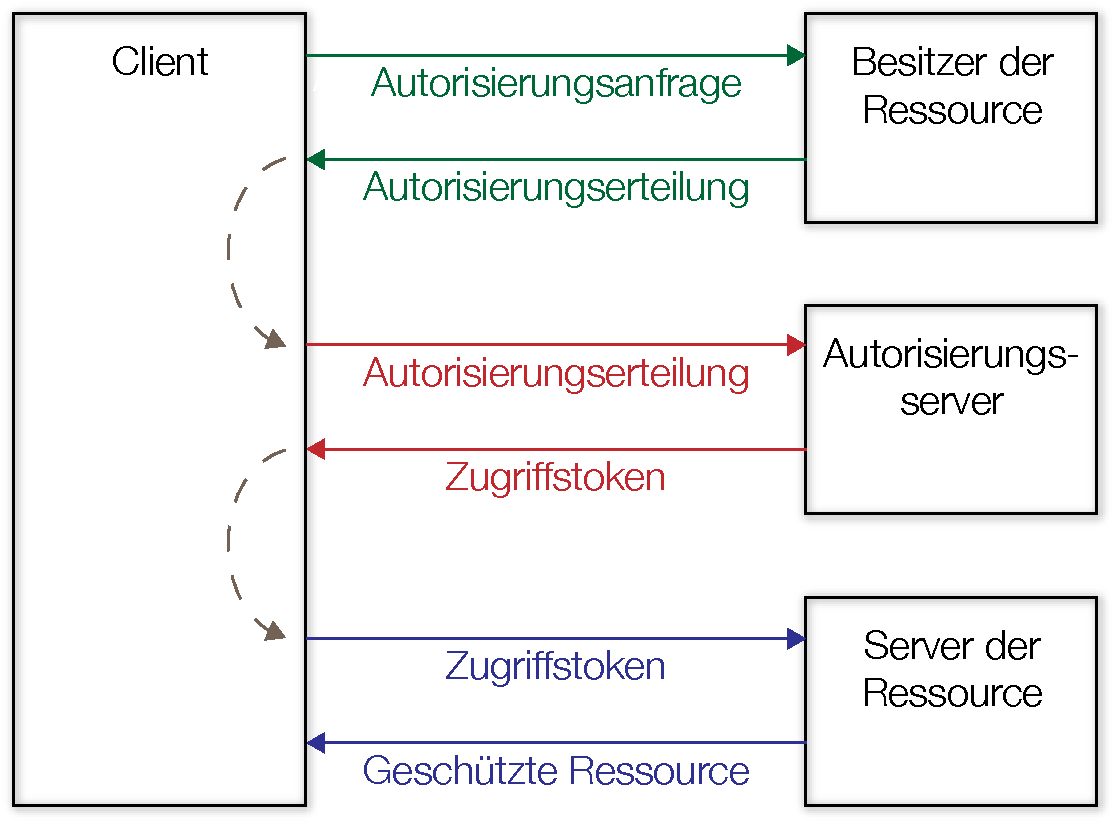
\includegraphics[width=.52\linewidth]{img/OAuth2}
		\caption{Protokollablauf bei OAuth 2 (übersetzt aus RFC 6749)}
	\end{figure}
\end{frame}
	
\subsection{\em JSON Web Tokens}
\begin{frame}{\insertsubsection}
	\begin{itemize}
		\item RFC 7519 \cite{RFC7519}
		\item simpler gegenüber \textit{OAuth}
		\item jeder Client kann verifizieren
		\item klein, daher via HTTP übertragbar
		\item kann auch von Browsern geparsed werden
	\end{itemize}
\end{frame}
	
\begin{frame}{\insertsubsection}{}%

\begin{figure}
	\framebox[.8\linewidth]{\parbox{.75\linewidth}%
{\color{red}\tt\footnotesize\{\\
		\hspace*{2em}"alg": "RS256",  \textcolor{gray}{// Verschlüsselungsalgorithmus}\\
		\hspace*{2em}"typ": "JWT" \textcolor{gray}{// „JSON Web Token“, offen für weitere}\\
\}}}
\caption{JWT-Header}
\end{figure}

\begin{figure}
	\framebox[.8\linewidth]{\parbox{.75\linewidth}%
{\color{violet}\tt\footnotesize\{\\
		\hspace*{2em}"thema": "Microservices und Sicherheit",\\
		\hspace*{2em}"modul": "Entwicklung verteilter Systeme",\\
		\hspace*{2em}"kursnr": "64-400"\\
	\}}}
\caption{JWT-Payload}
\end{figure}

\end{frame}

\begin{frame}{\insertsubsection}
	\begin{figure}
		{\tt \textcolor{red}{
				eyJhbGciOiJSUzI1NiIsInR5cCI6IkpXVCJ9}.\textcolor{violet}{eyJ0aG\\
				VtYSI6Ik1pY3Jvc2VydmljZXMgdW5kIFNpY2hlcmhla\\
				XQiLCJtb2R1bCI6IkVudHdpY2tsdW5nIHZlcnRlaWx0\\
				ZXIgU3lzdGVtZSIsImt1cnNuciI6IjY0LTQwMCJ9}.\textcolor{blue}{gb\\
				0y7zl4-IIZrRdWD14UaSGPz34vXqAPecoyQVeOrntFx\\
				PSkhryDHn2ts3Wn7XyHjli1HDdLZbqV5f1SzHNKZfz\_\\
				Ww8Tl2xzKLURpX9QxuI2PvFQZF0bQ7PeKqmZD7OU4eI\\
				4y9L6srzedEjsDDISbaFXTaIJp\_j1JtM9XTtEgi2Vy9\\
				TAIZczCacnxuJgxd-Nk40k6KgnFPz1ETIu9G3JyyMxP\\
				Enh1pw7EzIefJnRaaswC0K1evjQFK6dFvIlgXuevM3u\\
				gZcI7lA2f1PeMud1fkZu3yaw27jeeLZRU1WiRhMV9EB\\
				5elsYiscnpoVjuEk4C8T-p3oji43zf1IT7XvBiQ}}
		\caption{Vollständiges \textit{JSON Web Token}}
	\end{figure}
\end{frame}

\subsection{Integrität}
\begin{frame}{\insertsubsection}
	\begin{itemize}
		\item \textbf{Datenintegrität}:\\
			Vollständigkeit \& Korrektheit der Daten
		\item \textbf{Systemintegrität}:\\
			korrekte Funktionsweise des Systems
	\end{itemize}
	\vspace*{1cm}
	\pause
	Vorgestellte Verfahren:
	\begin{itemize}
		\item Verschlüsselung
		\item Integrationstests
	\end{itemize}
\end{frame}

\subsection{Integrationstests für Microservices}
\begin{frame}{\insertsubsection}
	\begin{figure}[h]
		\centering
		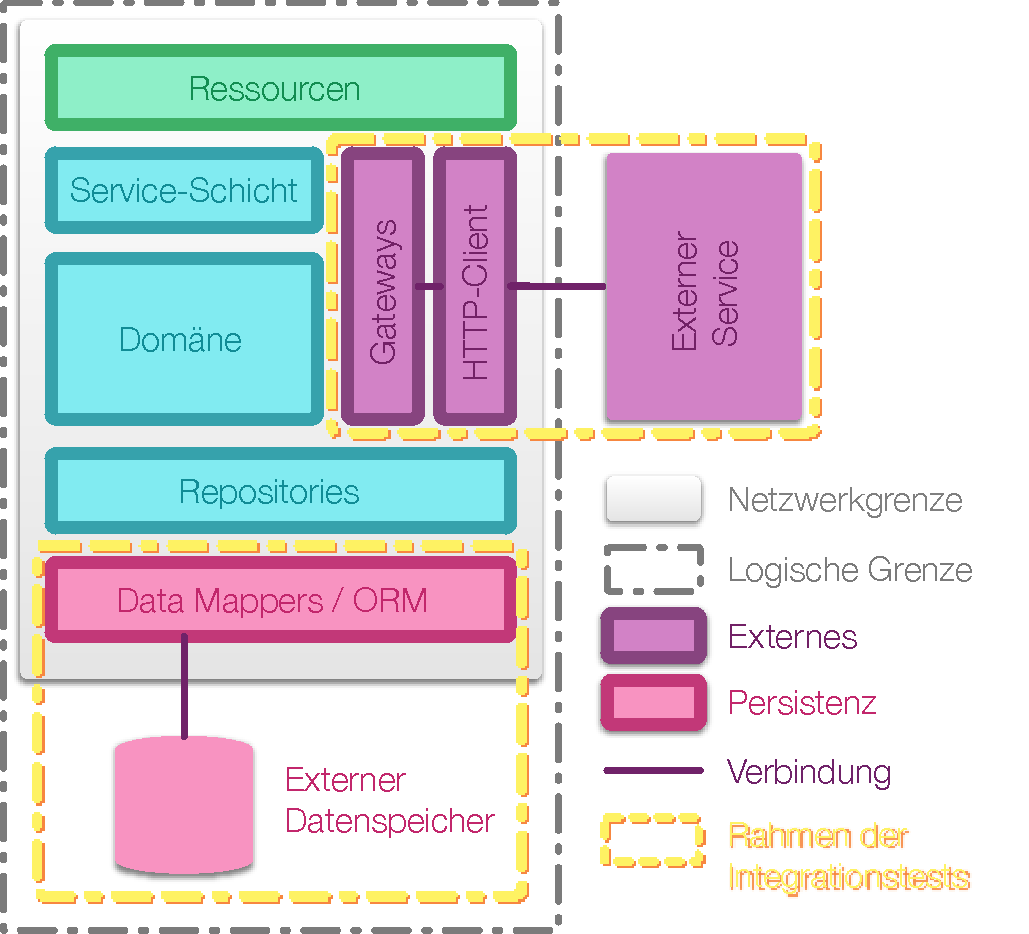
\includegraphics[width=.6\linewidth]{img/inte}
		\caption{Integrationstests in einer Microservice-Architektur (Clemson, 2014)}
		\label{fig:integrationstests}
	\end{figure}
\end{frame}

\subsection{Verfügbarkeit}
\begin{frame}{\insertsubsection}
	\begin{itemize}
		\item Systeme stets betriebsbereit
		\item zeitgerechter Zugriff auf Daten jederzeit möglich
	\end{itemize}
	\vspace*{1cm}
	\pause
	Vorgestellte Verfahren:
	\begin{itemize}
		\item horizontale Skalierung \& Lastverteilung
		\item \textit{Bakerstreet}
	\end{itemize}
\end{frame}


\subsection{Horizontale Skalierung \& Lastverteilung}

\subsection{\em Bakerstreet}
\begin{frame}{\insertsubsection}
	\begin{figure}
		\centering
		\includegraphics[width=.65\linewidth]{img/clientloadbal}
		\caption{Schematische Darstellung von clientseitiger Lastverteilung (aus Li, 2015)}
		\label{fig:clientseitige_lastverteilung}
	\end{figure}
\end{frame}

\section{Zusammenfassung}

% Literatur
\section{\bibname}
\begin{frame}[allowframebreaks]{\bibname}
	\AtBeginSection{}
	\nocite{*}
	\bibliographystyle{apacite}
	\bibliography{bib}
\end{frame}
\begin{frame}[allowframebreaks]{Bildquellen}
\end{frame}

\section{Demo und Diskussion}

\end{document}